\subsubsection{Proceso: Realizar gráfica 2D}

\begin{itemize}
	\item \textbf{O1:} Busca los valores de los atributos a partir del nombre y del nombre del juego, y consigue la tupla fecha, valor, nombre de jugador.
\end{itemize}

\begin{figure}[H]
	\centering
	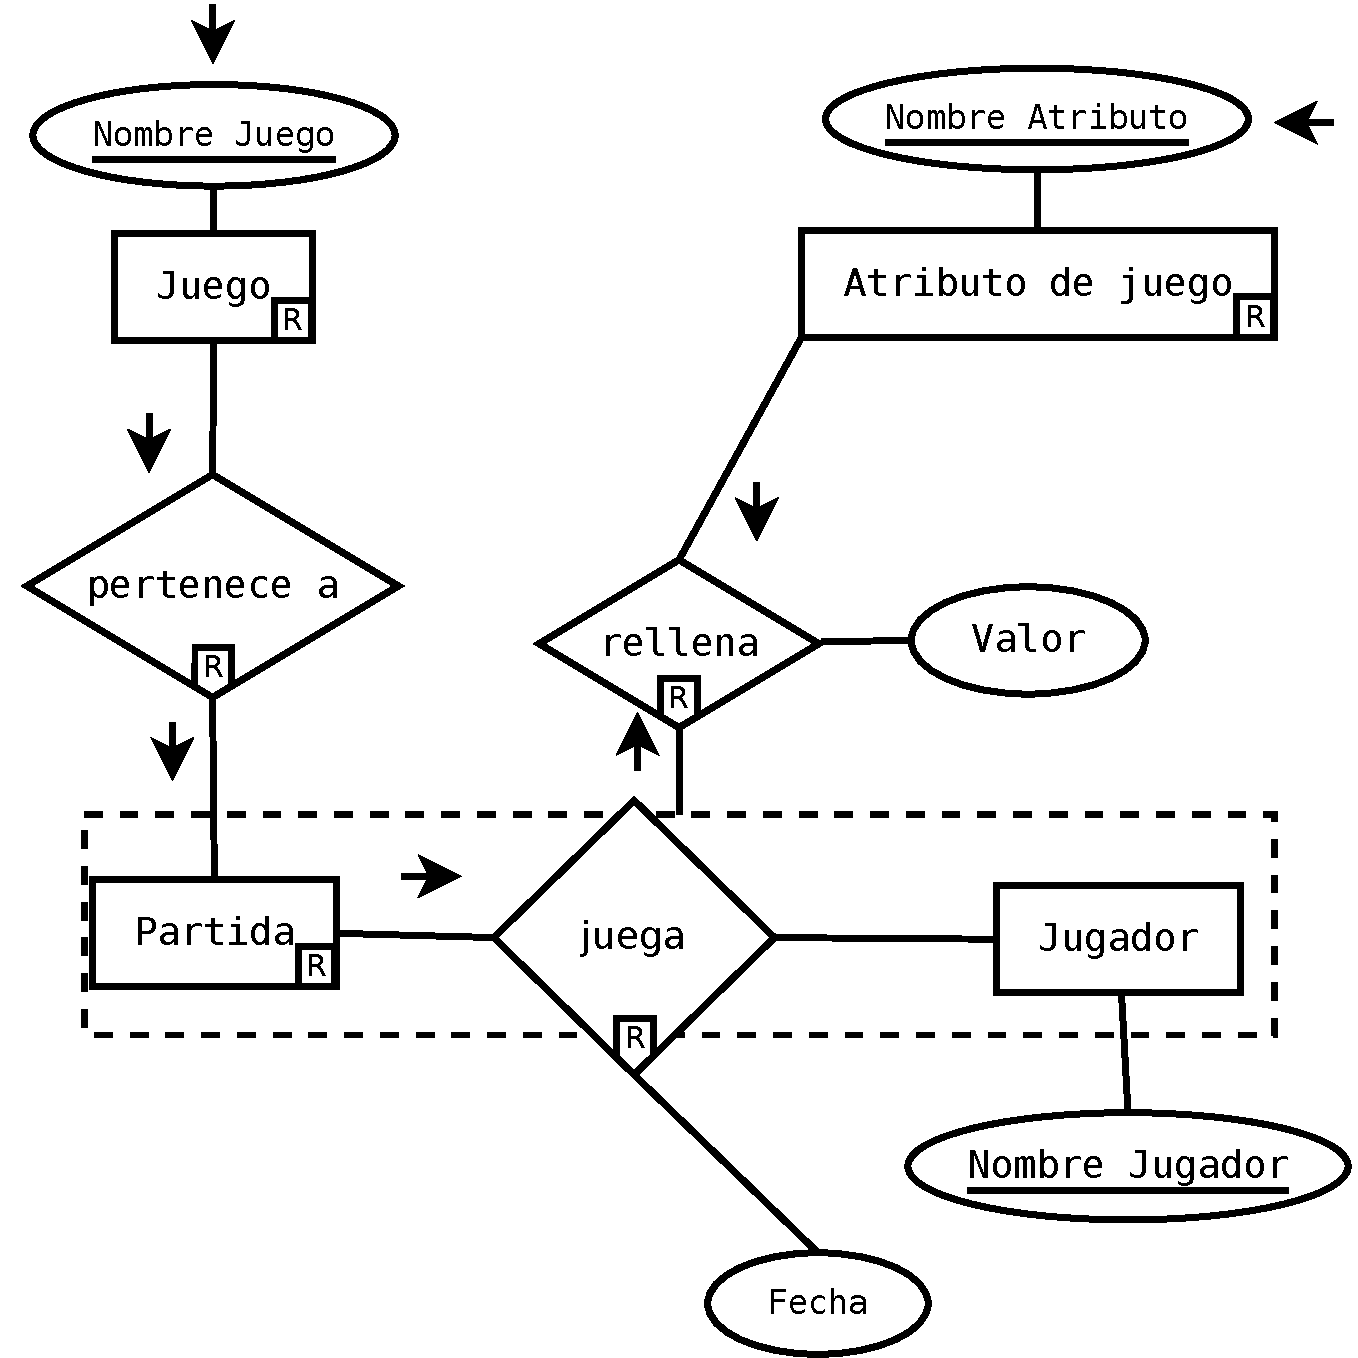
\includegraphics[width=0.5\linewidth]{../Diagramas/pdf/OpEstadisticas3.pdf}
	\caption{Esquema de navegabilidad  O1 del proceso 4.1}
	
	\label{fig:O4.1}
\end{figure}
 \begin{itemize}
 	\item \textbf{O2:} Con los valores anteriores, se ha realizado una gráfica que con esta operación insertamos. Conseguimos el usuario que está haciendo la estadística, la imagen de ella y su id, y la insertamos de forma correcta en la base de datos.
 \end{itemize}

\begin{figure}[H]
	\centering
	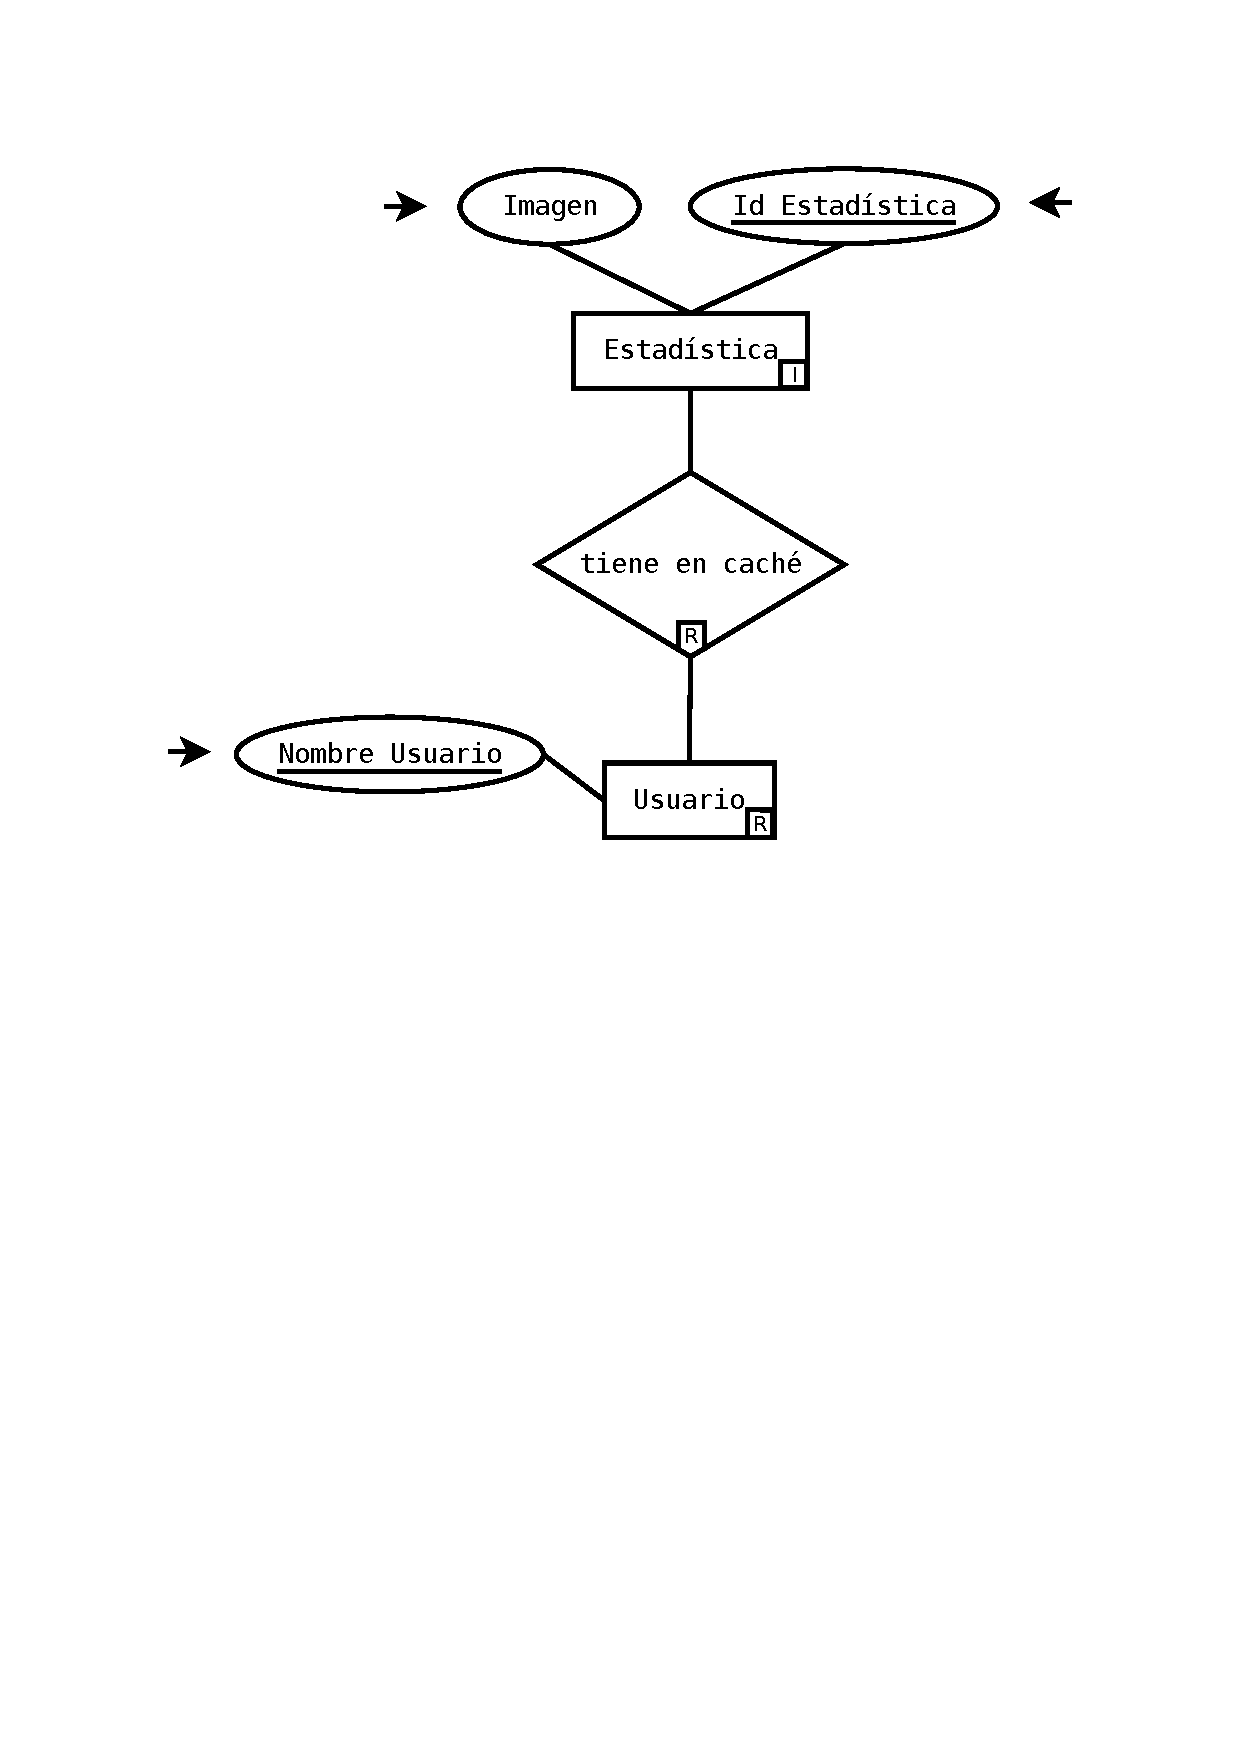
\includegraphics[width=0.5\linewidth]{../Diagramas/pdf/OpEstadisticas1-2.pdf}
	\caption{Esquema de navegabilidad  O2 del proceso 4.1}
	
	\label{fig:O4.12}
\end{figure}

